\begin{enumerate}
\item In \ref{Figure 2}, $PQ$ is a chord of a circle with centre $O$ and $PT$ is a tangent. If $\angle QPT = 60 \degree,$ Find $\angle PRQ $.
\begin{figure}[h!]
	\centering
    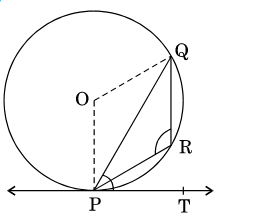
\includegraphics[width=\columnwidth]{figs/cbse_30_3_2.png}
	\label{Figure 2}
\end{figure}
\item The points 
\begin{align*}
 \vec{A}&= \myvec{4 \\ 7}\\  
 \vec{B}&=\myvec{p \\ 3}\\  
 \vec{C}&=\myvec{7 \\ 3}
\end{align*}
are the vertices of a right triangle, right-angled at $ \vec{B} $. Find the value of $p$.
\item In Figure \ref{Figure 3}, two tangents $RQ$ and $RP$ are drawn from an external point $R$ to the circle with centre $O$. If $\angle PRQ = 120 \degree,$ then prove that $OR = PR + RQ$.
  \begin{figure}[h!]
	\centering
    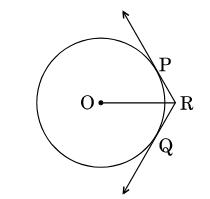
\includegraphics[width=\columnwidth]{figs/cbse_30_3_3.png}
	\label{Figure 3}
\end{figure}
\item In Figure \ref{Figure 4}, a triangle $ABC$ is drawn to circumscribe a circle of radius $3$ cm, such that the segments $BD$ and $DC$ are respectively of lengths $6$ cm  and $9$ cm. If the area of $\triangle \text{ABC is }54 cm^2$, then find the lengths of sides $AB$ and $AC$.
\begin{figure}[h!]
	\centering
    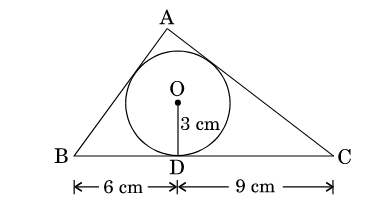
\includegraphics[width=\columnwidth]{figs/cbse_30_3_4.png}
	\label{Figure 4}
\end{figure}
\item Find the relation between x and y if the points 
\begin{align*}
\vec{A}&=\myvec{x \\ y}\\ 
\vec{B}&=\myvec{-5\\7}\\
\vec{C}&=\myvec{-4\\5} 
\end{align*}
are collinear.
\item Find the coordinates of a point $P$ on the line segment joining
\begin{align*}
\vec{A} &= \myvec{1\\2}\\
\vec{B} &= \myvec{6\\7}
\end{align*}
such that AP = $\dfrac{2}{5}$AB.
\item Find the values of $k$ for which the points
\begin{align*}
\vec{A} &= \myvec{k+1\\2k}\\
\vec{B} &= \myvec{3k\\2k+3}\\
\vec{C} &= \myvec{5k-1\\5k}
\end{align*}
are collinear.
\item Prove that the lengths of the tangents drawn from an external point to a circle are equal.
\item Prove that the tangent drawn at the mid-point of an arc of a circle is parallel to the chord joining the end points of the arc.
\item Due to sudden floods, some welfare associations jointly requested the government to get $100$ tents fixed immediately and offered to contribute $ 50\% $ of the cost. If the lower part of each tent is of the form of a cylinder of diameter $4.2$ m and height $4$ m with the conical upper part of same diameter but of height $2.8$ m, and the canvas to be used costs \rupee $100$ per sq. m, find the amount, the associations will have to pay. What values are shown by these associations ? [Use $\pi=\dfrac{22}{7}$]
\item A hemispherical bowl of internal diameter $36$ cm contains liquid. This liquid is filled into $72$ cylindrical bottles of diameter $6$ cm. Find the height of the each bottle, if $10 \% $ liquid is wasted in this transfer.
\item A cubical block of side $10$ cm is surmounted by a hemisphere. What is the largest diameter that the hemisphere can have ? Find the cost of painting the total surface area of the solid so formed, at the rate of \rupee $5$ per $100$ sq. cm. [Use $\pi= 3.14$]
\item $504$ cones, each of diameter $3.5$ cm and height $3$ cm, are melted and recast into a metallic sphere. Find the diameter of the sphere and hence find its surface area. [Use $\pi=\dfrac{22}{7}$]


\item Find the area of the minor segment of a circle of radius $14$ cm, when its central angle is $60 \degree.$ Also find the area of the corresponding major segment. [Use $\pi =\dfrac{22}{7}$]
\item In \ref{Figure 5}, $PQRS$ is a square lawn with side $PQ = 42$ metres. Two circular flower beds are there on the sides $PS$ and $QR$ with centre at $O$, the intersection of its diagonals. Find the total area of the two flower beds (shaded parts).
 \begin{figure}[h!]
	\centering
    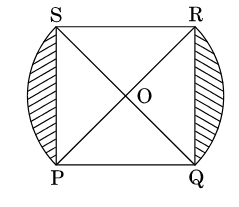
\includegraphics[width=\columnwidth]{figs/cbse_30_3_5.png}
	\label{Figure 5}
\end{figure}
\item From each end of a solid metal cylinder, metal was scooped out in hemispherical form of same diameter. The height of the cylinder is $10$ cm and its base is of radius $4.2$ cm. The rest of the cylinder is melted and converted into a cylindrical wire of $1.4$ cm thickness. Find the length of the wire. [Use $ \pi=\frac{22}{7} $]
\item The diagonal of a rectangular field is $16$ metres more than the shorter side. If the longer side is $14$ metres more than the shorter side, then find the lengths of the sides of the field.


\end{enumerate}
